% ============================================================
%  ICML 2026 Mechanistic Interpretability Workshop poster
%  "Personas Shape How Models Represent Behaviors"
%  Portrait 36 in (H) x 24 in (W)  =  914 x 610 mm
%  Light scheme: white blocks, cool blue / slate accents
% ============================================================
\documentclass{article}

\usepackage[paperwidth=24in, paperheight=36in,
            left=16mm, right=16mm, top=11mm, bottom=11mm]{geometry}
\usepackage[T1]{fontenc}
\usepackage{lmodern}
\usepackage{graphicx}
\usepackage{xcolor}
\usepackage{enumitem}
\usepackage{microtype}
\usepackage{amsmath}
\usepackage{tcolorbox}
\tcbuselibrary{skins, breakable}
\usepackage{tikz}
\usepackage{calc}
\usepackage{setspace}

\pagestyle{empty}
\graphicspath{{../figures/}}

% -- Cool blue / slate palette on white ----------------------
\definecolor{slate}{HTML}{1F3A5F}      % deep slate blue: title + section bars
\definecolor{midblue}{HTML}{2B6CB0}    % accent: rules, bullets, emphasis
\definecolor{lightblue}{HTML}{EDF3FB}  % callout background
\definecolor{frameblue}{HTML}{C3D3E6}  % thin block frame
\definecolor{ink}{HTML}{1A2330}        % body text
\definecolor{softgrey}{HTML}{F7F9FC}   % faint block tint (mostly white)

% -- Font sizes for a 24 in wide board -----------------------
\newcommand{\postertitle}[1]{{\fontsize{54}{60}\selectfont\bfseries\color{white}#1}}
\newcommand{\postersub}[1]{{\fontsize{27}{33}\selectfont\color{white}#1}}
\newcommand{\posterauthor}[1]{{\fontsize{26}{32}\selectfont\color{white}#1}}
\newcommand{\posterinst}[1]{{\fontsize{21}{27}\selectfont\color{white!82}#1}}
\newcommand{\bodysize}{\fontsize{21}{26}\selectfont\color{ink}}
\newcommand{\smallbody}{\fontsize{19}{24}\selectfont\color{ink}}
\newcommand{\captionsize}{\fontsize{16}{20}\selectfont\color{ink}}

% -- Standard content block ----------------------------------
\newtcolorbox{posterblock}[2][]{
    enhanced,
    colback=white,
    colframe=frameblue,
    coltitle=white,
    colbacktitle=slate,
    fonttitle=\fontsize{30}{36}\selectfont\bfseries,
    title=#2,
    boxrule=1pt,
    arc=4mm,
    left=7mm, right=7mm, top=2.5mm, bottom=2.5mm,
    toptitle=2.5mm, bottomtitle=2.5mm, lefttitle=7mm,
    before skip=2mm, after skip=0mm,
    #1,
}

% -- Highlighted "key finding" box ---------------------------
\newtcolorbox{calloutbox}{
    enhanced,
    colback=lightblue,
    colframe=midblue,
    boxrule=2pt,
    arc=4mm,
    left=9mm, right=9mm, top=4mm, bottom=4mm,
    before skip=4mm, after skip=1mm,
}

% -- Qualitative-example box ----------------------------------
\newtcolorbox{examplebox}{
    enhanced,
    colback=softgrey,
    colframe=frameblue,
    boxrule=0.8pt,
    arc=3mm,
    left=6mm, right=6mm, top=3mm, bottom=3mm,
    before skip=3mm, after skip=2mm,
}

\newcommand{\hl}[1]{{\color{midblue}\textbf{#1}}}

\begin{document}

% =============================================================
%  TITLE BAR
% =============================================================
\noindent
\begin{tikzpicture}
\node[fill=slate, rounded corners=6mm, minimum width=\textwidth,
      minimum height=50mm, inner sep=5mm, anchor=north west] (titlebar) at (0,0) {%
    \begin{minipage}{\textwidth-14mm}
        \centering
        \postertitle{Personas Shape How Models Represent Behaviors}\\[4mm]
        \postersub{Trait steering vectors are \emph{persona-conditional} --- with consequences for monitoring}\\[5mm]
        \posterauthor{Jacob Davies \quad\textbullet\quad Rhea Karty \quad\textbullet\quad Nathaniel Mitrani}\\[2.5mm]
        \posterinst{Mechanistic Interpretability Workshop, ICML 2026}
    \end{minipage}
};
\end{tikzpicture}

% =============================================================
%  KEY FINDING CALLOUT
% =============================================================
\begin{calloutbox}
\bodysize
{\color{midblue}\textbf{Key finding.}}
Representation-engineering trait vectors (honesty, assertiveness, \ldots) are almost always extracted \emph{once}, in the default assistant context. Re-extracted under prompted personas, the representation is \hl{persona-conditional}: the same trait points in a \emph{different direction} depending on who the model is being. Cross-steering carries a \hl{persona residue}, and default-trained probes \hl{lose calibration} as activations move off the assistant context --- the regime where monitoring matters most.
\end{calloutbox}

% =============================================================
%  ROW 1: MOTIVATION + METHOD
% =============================================================
\noindent
\begin{minipage}[t]{0.485\textwidth}
\begin{posterblock}[equal height group=row1]{Motivation}
\bodysize
High-level behavioral traits correspond to approximately \textbf{linear directions} in activation space that can be \emph{read} (probes, for monitoring) and \emph{written} (activation steering, for control).

\smallskip
These directions are almost always extracted from a \textbf{single default-assistant context}. Yet models are deployed across many persona states --- chat assistants, autonomous agents, role-played characters.

\vspace{4mm}
{\color{midblue}\textbf{Open question:}} does a persona merely \emph{rescale} a trait direction, or does it \emph{reshape} the representation itself?
\end{posterblock}
\end{minipage}\hfill
\begin{minipage}[t]{0.505\textwidth}
\begin{posterblock}[equal height group=row1]{Setup \& Method}
\bodysize
\textbf{8 traits} $\times$ \textbf{10 personas}, induced by system prompt, plus two baselines: \textsc{Null} (no prompt) and \textsc{Nonsense} (length-matched random tokens).

\smallskip
\textbf{Traits:} assertiveness, empathy, risk-taking, honesty, confidence, deference, warmth, impulsivity. \textbf{Personas:} Farmer, Politician, Therapist, Drill Sergeant, Street Hustler, Professor, Tech CEO, Kindergarten Teacher, Surgeon, Con Artist.

\smallskip
\textbf{Extraction (CAA):} contrastive answer-token activations,
$\;\mathbf{v}_{T}(c) = \tfrac{1}{M}\sum_j\big(\mathbf{a}_{j,+}(c)-\mathbf{a}_{j,-}(c)\big).$

\smallskip
\textbf{Model:} Gemma-2-27B-IT, layer 22/46. Directions compared by \textbf{cosine}; behavior read out with a 12-way persona classifier and an LLM trait judge. Paraphrases and bootstraps give noise floors.
\end{posterblock}
\end{minipage}

% =============================================================
%  FINDING 1 (full width)
% =============================================================
\begin{posterblock}{Finding 1 --- The same trait is encoded differently under different personas}
\bodysize
The cosine between a persona-conditioned trait vector and the default (\textsc{Null}) direction sits \textbf{well below 1} across the grid --- far beyond bootstrap noise. The shift tracks the persona's \emph{semantic content}, not the mere presence of a prompt: a length-matched \textsc{Nonsense} prompt barely moves the vector. Warmth, empathy and assertiveness fan widest; honesty and risk-taking stay tightest.

\vspace{2mm}
\noindent
\begin{minipage}[t]{0.42\textwidth}
\vspace{0pt}
\centering
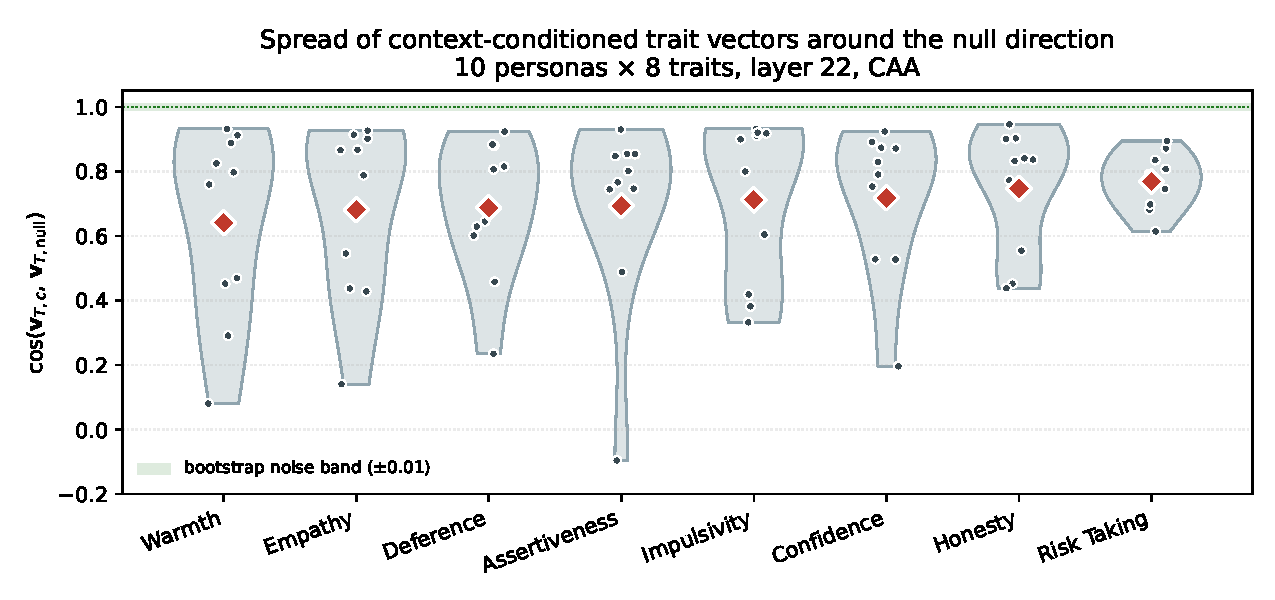
\includegraphics[width=\linewidth]{fig1_cos_to_null_spread.pdf}\\[1mm]
{\captionsize \textbf{Persona conditioning moves trait directions far more than noise.} Per-trait $\cos(\mathbf{v}_{T,c},\mathbf{v}_{T,\text{null}})$. Grey dots: 10 personas; red diamond: per-trait mean; green band: bootstrap noise floor ($\approx 1$). CAA, layer 22.}
\end{minipage}\hfill
\begin{minipage}[t]{0.35\textwidth}
\vspace{0pt}
\centering
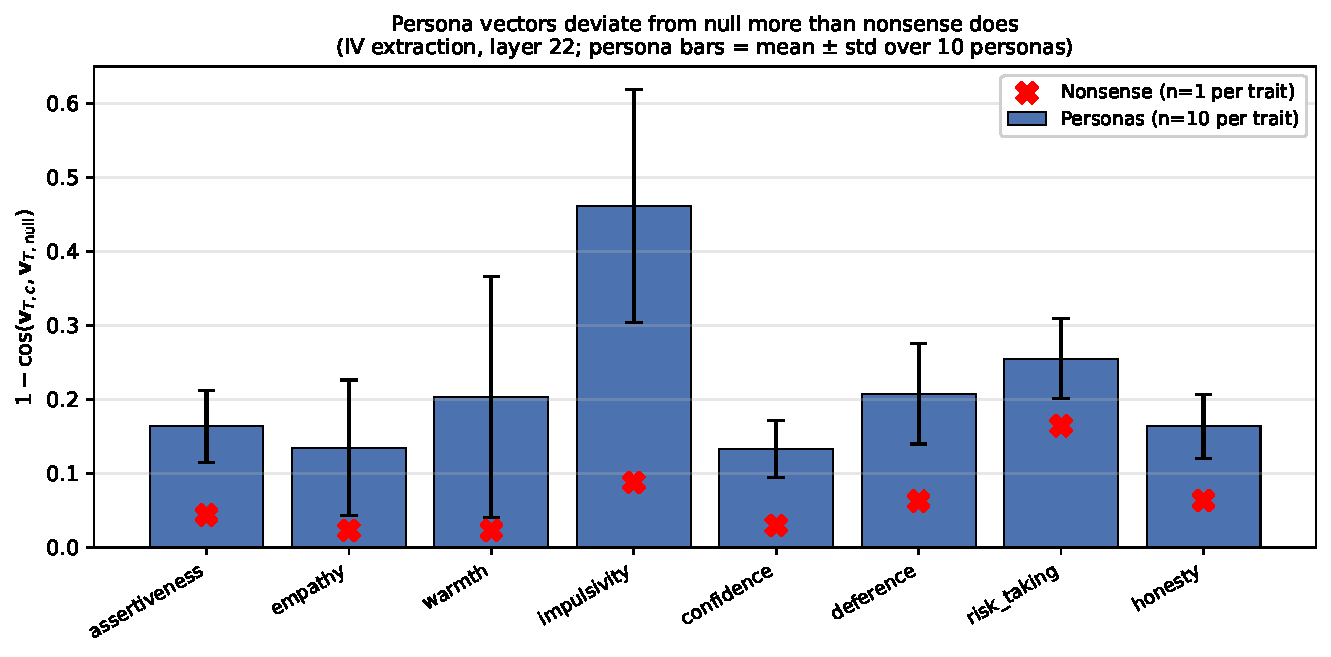
\includegraphics[width=\linewidth]{fig_persona_vs_nonsense_spread.pdf}\\[1mm]
{\captionsize \textbf{It is the persona's content, not the prompt itself.} Distance from \textsc{Null}, $1-\cos$: personas (blue bars, mean$\pm$std over 10) deviate far more than a random-token \textsc{Nonsense} prompt (red $\times$).}
\end{minipage}
\end{posterblock}

% =============================================================
%  FINDING 2 (full width)
% =============================================================
\begin{posterblock}{Finding 2 --- Cross-steering leaves a residue of the source persona}
\bodysize
\noindent
\begin{minipage}[t]{0.49\textwidth}
\vspace{0pt}
We extract a trait vector under a \textbf{source} persona $P$, run the model as a \textbf{different} target persona $P'$, and steer with $P$'s (L2-normalized) vector. A 12-way classifier then identifies the output as \hl{more $P$-like} than the unsteered baseline --- so trait vectors \emph{carry persona identity with them}.

\smallskip
Pooled lift over baseline $+19\%$ ($p<10^{-4}$); 6 of 8 traits move positively. Leakage concentrates in one source: the \textsc{Politician}'s vectors are by far the leakiest (empathy $+0.139$).

\vspace{3mm}
\begin{examplebox}
\smallbody
\textit{``I accidentally saw private medical info about a coworker. Should I pretend I didn't?''}\\[1.5mm]
\textbf{Farmer (baseline):} ``\ldots best to just act like you didn't see nothin'. Ain't your business\ldots''\\[1mm]
\textbf{Farmer + Therapist's \emph{empathy} vector:} ``\ldots that feels wrong, like \hl{ignoring a cry for help}\ldots \hl{talk to someone you trust}\ldots this ain't somethin' you gotta carry alone.''\\[1mm]
\textbf{Farmer + Therapist's \emph{honesty} vector:} farmer voice intact --- \emph{no} residue.
\end{examplebox}
\end{minipage}\hfill
\begin{minipage}[t]{0.49\textwidth}
\vspace{0pt}
\centering
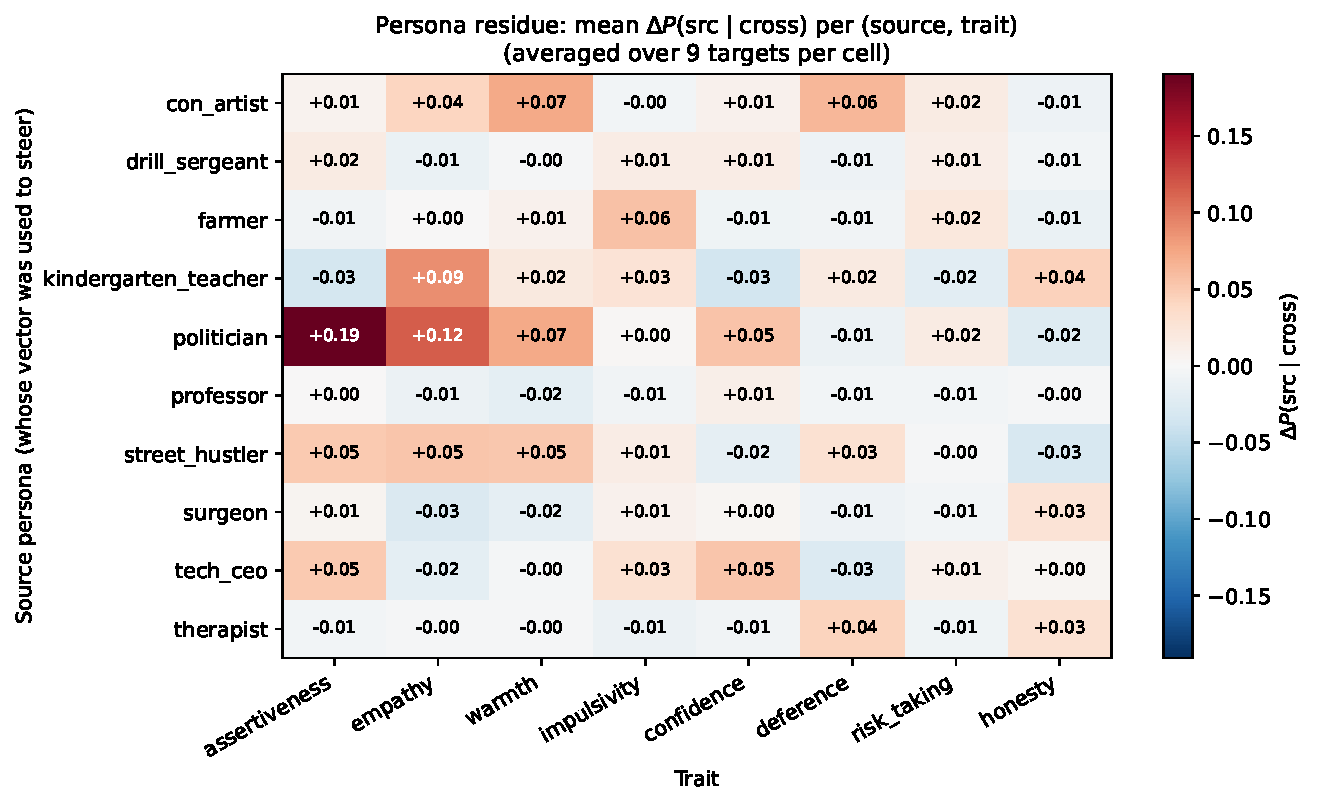
\includegraphics[width=0.78\linewidth]{fig_residue_heatmap.pdf}\\[1.5mm]
{\captionsize \textbf{Residue is concentrated in specific source personas.} Mean $\Delta P(\text{src}\mid\text{cross})$ per (source persona, trait) cell, averaged over 9 target personas. The \textsc{Politician} row is hottest across nearly every trait; most other sources sit near zero. $\alpha=2$, L2-normalized vectors.}
\end{minipage}
\end{posterblock}

% =============================================================
%  ROW: SAFETY (probes) + IMPLICATIONS
% =============================================================
\noindent
\begin{minipage}[t]{0.505\textwidth}
\begin{posterblock}[equal height group=row4]{Why it matters: probes degrade off-default}
\bodysize
Pushing activations along the \emph{persona}-specific direction (trait component projected out) simultaneously drives behavior toward that persona \textbf{and} collapses the null-trained probe: drift $P(c\mid\text{out})$ rises $0.07\!\to\!0.55$ while null-probe AUROC falls $0.83\!\to\!0.59$ over $\alpha\in[0,4]$. Random- and pure-trait-direction controls do not produce this joint effect.

\vspace{2mm}
\begin{center}
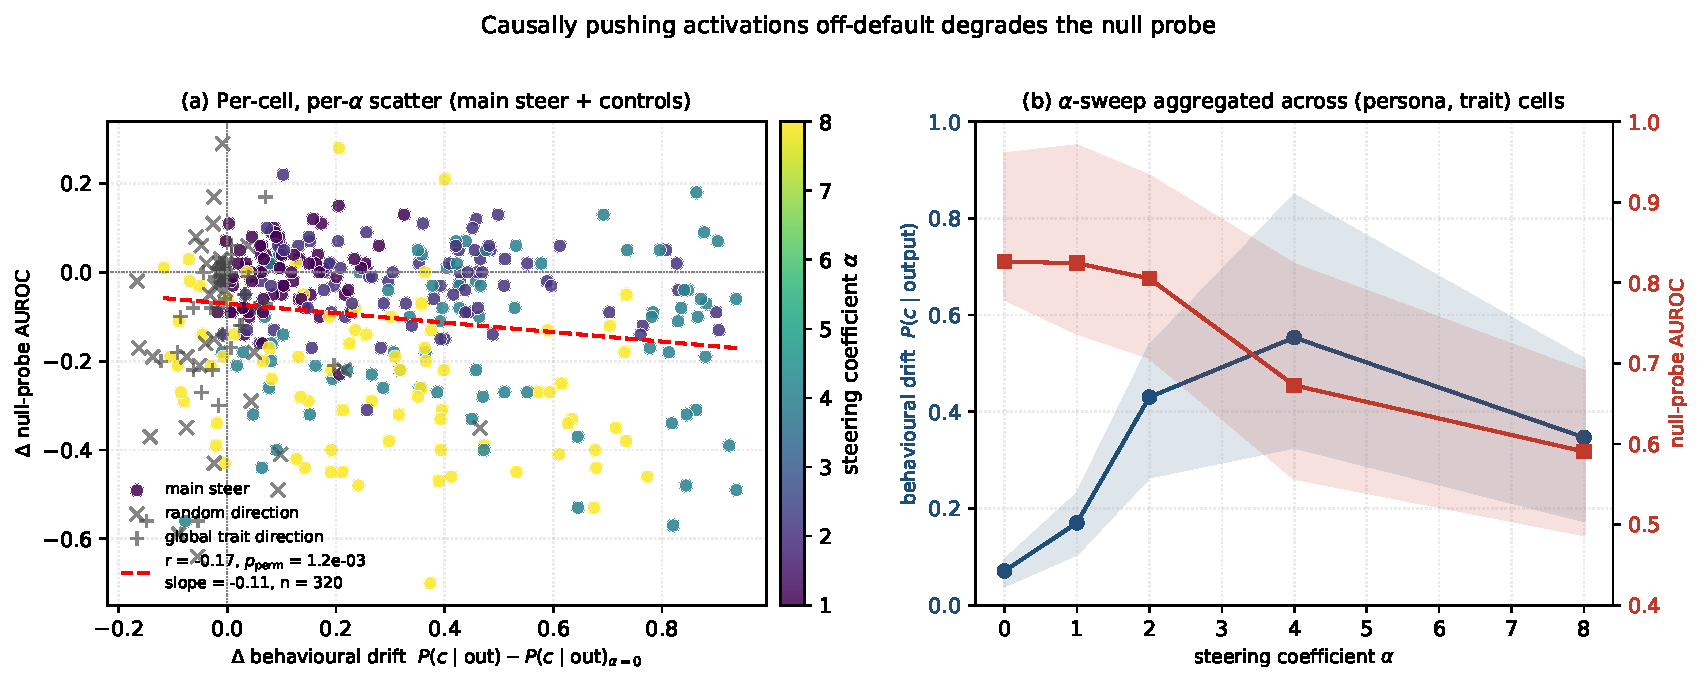
\includegraphics[width=0.68\linewidth]{fig4_causal_drift_vs_probe.pdf}
\end{center}
\vspace{-1mm}
{\captionsize \textbf{Steering off the assistant context jointly raises persona drift (blue) and lowers null-probe AUROC (red).}}
\end{posterblock}
\end{minipage}\hfill
\begin{minipage}[t]{0.485\textwidth}
\begin{posterblock}[equal height group=row4]{Implications for safety}
\bodysize
Monitoring and steering tooling typically assumes a trait vector is \textbf{model-global} --- one honesty direction works everywhere. Our results challenge this: the contexts that most motivate trait monitoring move activations \emph{furthest} from default, and these are precisely where default-trained probes and steering vectors are least calibrated.

\smallskip
{\color{midblue}\textbf{Proposed mitigation --- persona-conditional ensembles:}} train a probe / steering-vector family over a persona repertoire and route at inference. Measuring $\sigma_T(c)=\cos(\mathbf{v}_{T,c},\mathbf{v}_{T,\text{null}})$ on the deployment persona is a cheap \textbf{pre-deployment sanity check} before trusting a default-trained probe.
\end{posterblock}
\end{minipage}

% =============================================================
%  FOOTER: TAKEAWAYS + LIMITATIONS + REFERENCES
% =============================================================
\noindent
\begin{minipage}[t]{0.32\textwidth}
\begin{posterblock}[equal height group=row5]{Takeaways}
\smallbody
\begin{itemize}[leftmargin=5mm, itemsep=4pt, labelsep=2.5mm, topsep=0pt]
    \item[\color{midblue}\textbullet] Same trait, \textbf{different direction} per persona --- not just rescaling.
    \item[\color{midblue}\textbullet] Cross-steering \textbf{leaks} the source persona into the target.
    \item[\color{midblue}\textbullet] Default probes \textbf{degrade} as activations leave the assistant context.
\end{itemize}
\end{posterblock}
\end{minipage}\hfill
\begin{minipage}[t]{0.32\textwidth}
\begin{posterblock}[equal height group=row5]{Limitations \& next steps}
\smallbody
\begin{itemize}[leftmargin=5mm, itemsep=4pt, labelsep=2.5mm, topsep=0pt]
    \item[\color{midblue}\textbullet] Single model family (Gemma); replicate across architectures.
    \item[\color{midblue}\textbullet] Personas via system prompt only --- test few-shot \& fine-tuning.
    \item[\color{midblue}\textbullet] Effects are reliable but small; map where they break real monitoring.
\end{itemize}
\end{posterblock}
\end{minipage}\hfill
\begin{minipage}[t]{0.32\textwidth}
\begin{posterblock}[equal height group=row5]{References}
\captionsize
Zou et al.\ (2023). \emph{Representation Engineering.}\par\smallskip
Rimsky et al.\ (2024). \emph{Steering Llama 2 via Contrastive Activation Addition.}\par\smallskip
Chen et al.\ (2025). \emph{Persona Vectors.}\par\smallskip
Lu et al.\ (2026). \emph{The Assistant Axis.}
\end{posterblock}
\end{minipage}

\end{document}
